\chapter{Background Theory}
\label{chap3}

\section{Introduction}
This chapter introduces the technical concepts behind the system built 
in this thesis. It begins with the transformer architecture that modern 
language models are built on, then describes the two generative models 
used in the experiments and the quantization technique that makes them 
feasible on a single GPU. It then covers dense semantic embeddings and 
vector retrieval, the three document chunking strategies compared in 
the experiments, the two conversational memory mechanisms evaluated, 
and finally the metrics used to measure system output quality.

\section{The Transformer Architecture}

The transformer, introduced by Vaswani et al. in 2017 
\cite{vaswani2017attention}, replaced recurrent architectures with a 
mechanism based entirely on attention. Rather than processing tokens 
one at a time in sequence, the transformer computes relationships 
between all positions in the input in parallel, removing the 
information bottleneck that limited recurrent models on long documents.

The core operation is scaled dot-product attention. Given three 
matrices — queries $Q$, keys $K$, and values $V$ derived from the 
input — the output is:

\begin{equation}
    \text{Attention}(Q, K, V) = 
    \text{softmax}\!\left(\frac{QK^\top}{\sqrt{d_k}}\right)V
\end{equation}

where $d_k$ is the dimension of the key vectors. The division by 
$\sqrt{d_k}$ prevents the dot products from growing large in magnitude, 
which would push the softmax into regions with near-zero gradients. 
The result is a weighted combination of value vectors, where the weights 
express how relevant each position is to every other position in the 
input.

\begin{figure}[!h]
    \centering
    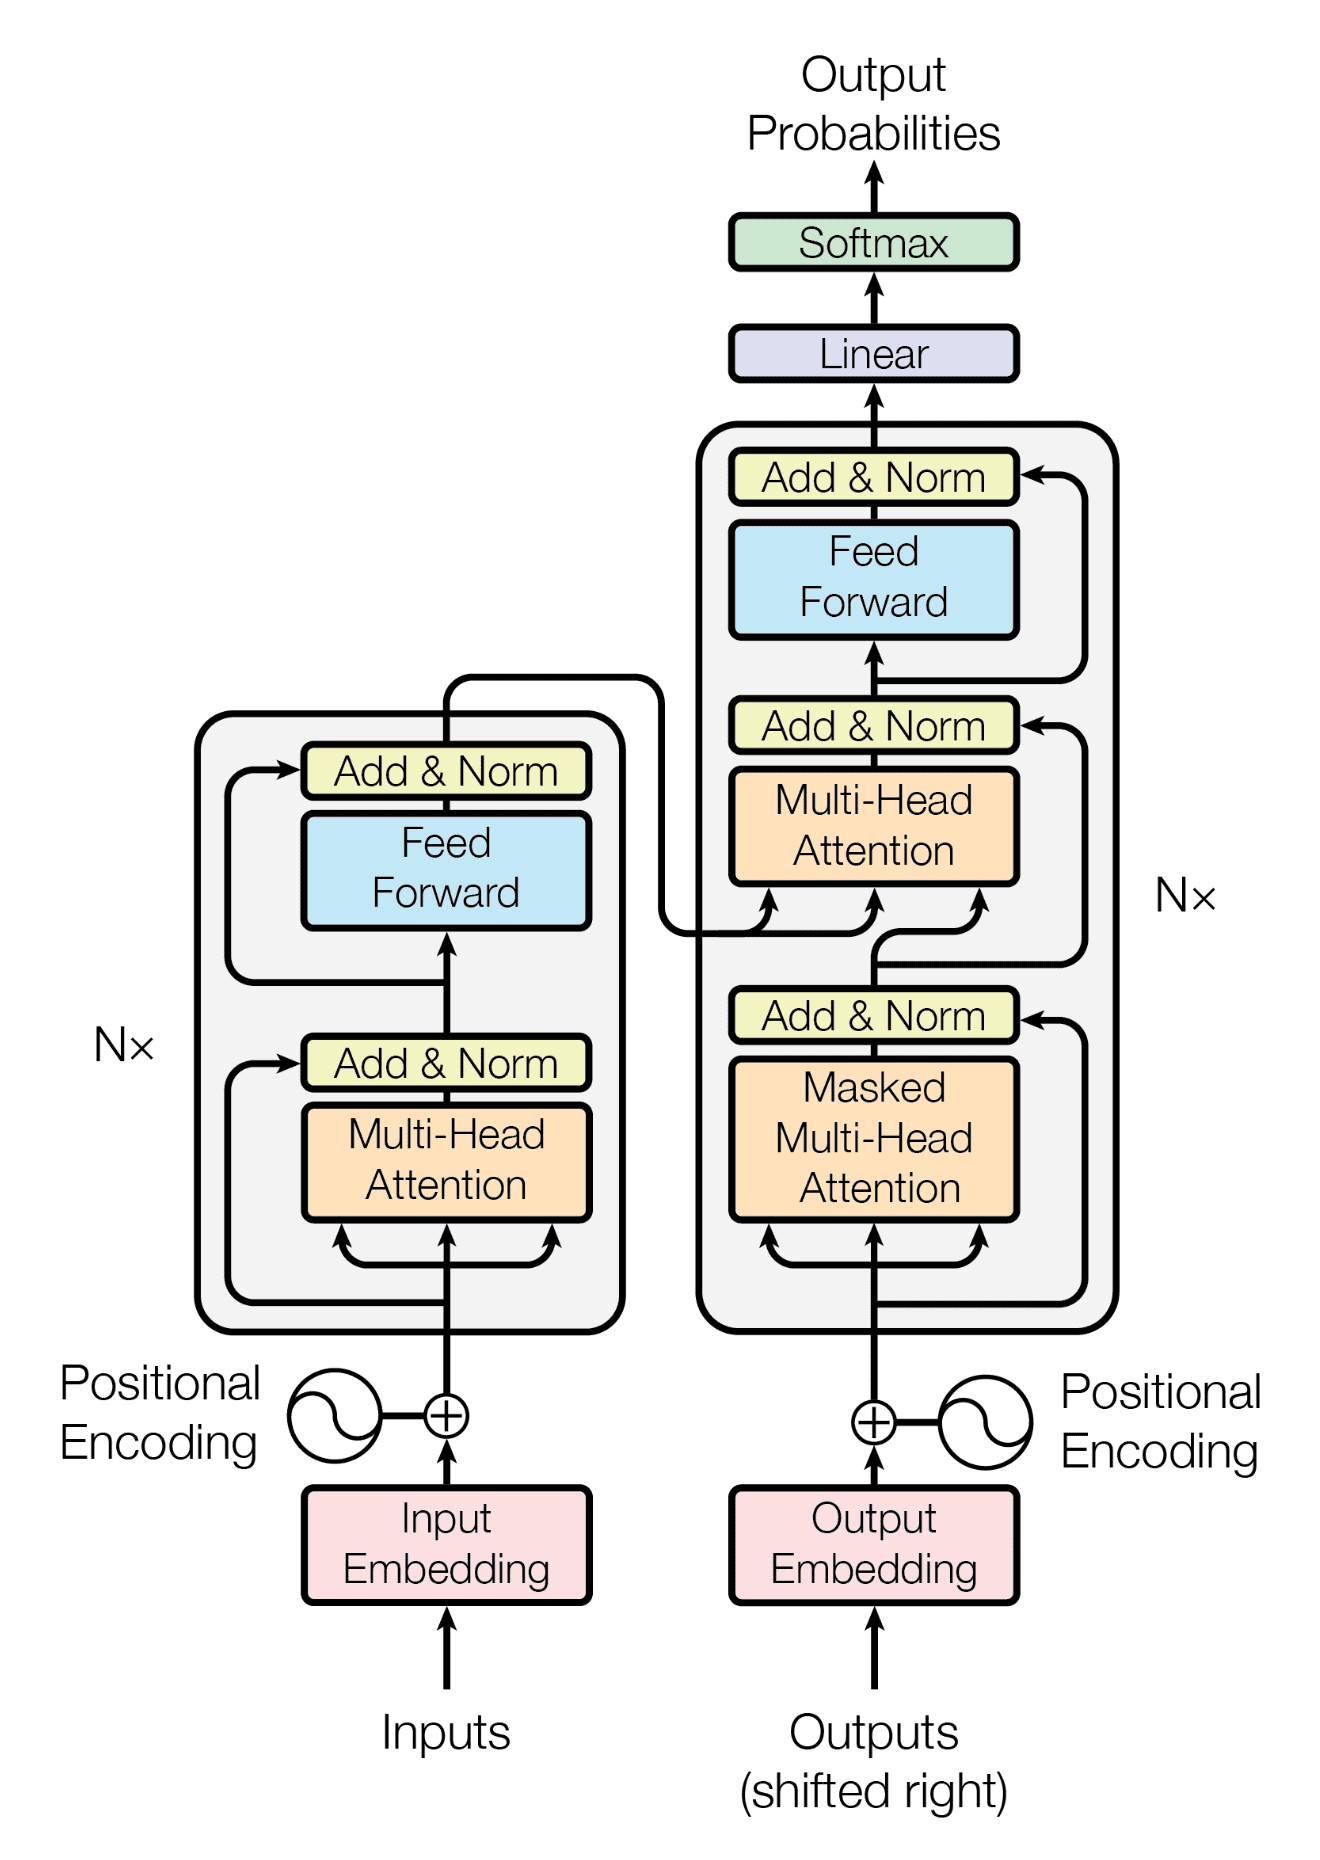
\includegraphics[width=0.5\linewidth]{figures/transformers.png}
    \caption{Transformers architecture.}
    \label{fig:transformer}
\end{figure}

In practice, several attention heads run in parallel and their outputs 
are concatenated, allowing the model to attend to different aspects of 
the input at the same time. This multi-head attention sits alongside 
feed-forward layers and residual connections inside each transformer 
block. BERT \cite{devlin2019bert} stacked 12 such blocks in an 
encoder-only configuration, pre-training on masked language modeling 
to produce contextual representations that became the starting point 
for most subsequent NLP work. Encoder-only models excel at 
classification and retrieval but cannot generate text. Generative 
systems require decoder-based models, described in the next section.

\section{Large Language Models}

\subsection{Decoder-Only Generation}

Decoder-only transformers are trained autoregressively: the model 
predicts the next token given all previous tokens, then appends that 
prediction and repeats until the output is complete. A causal attention 
mask enforces this by preventing any position from attending to tokens 
that come after it in the sequence.

Training these models at scale — billions of parameters on trillions 
of tokens — produces systems that can follow instructions and answer 
questions without task-specific fine-tuning. Instruction-tuned variants 
go a step further: after pre-training, the model is refined using 
reinforcement learning from human feedback (RLHF), which adjusts its 
outputs toward responses that human raters judge as correct and helpful.

\subsection{Llama 3.1}

Meta's Llama family is one of the most widely used open-weight 
generative model series. Llama~2 \cite{touvron2023llama2} released 
7B, 13B, and 70B parameter models alongside instruction-tuned variants 
trained via RLHF. Llama~3.1 \cite{meta2024llama3} extended the series 
with a context window of 128,000 tokens, compared to the 4,096-token 
limit of Llama~2. For legal contracts, which routinely span tens of 
thousands of words, this matters: a clause near the end of a document 
remains accessible to the model during generation rather than being 
truncated out of the input. The 8B parameter variant is used throughout 
this thesis.

\subsection{Mistral 7B}

Jiang et al. released Mistral 7B in 2023 \cite{jiang2023mistral}. 
Despite having fewer parameters than Llama~2~13B, it matched or 
exceeded it on most standard benchmarks. Two architectural decisions 
account for this. Grouped query attention shares key and value matrices 
across multiple attention heads instead of computing a separate pair 
for each, which reduces the memory occupied by the key-value cache 
during inference. Sliding window attention limits each token to 
attending within a fixed window of past positions rather than the 
entire sequence, keeping computation cost proportional to the window 
size rather than the full context length. Both choices lower the 
per-token cost of inference without removing the model's ability to 
reason over long passages.

\subsection{4-Bit NF4 Quantization}

A 7B or 8B parameter model stored in 32-bit floating point requires 
roughly 28--32~GB of GPU memory. Quantization reduces this by 
representing weights at lower precision. The NF4 format, introduced 
by Dettmers et al. as part of QLoRA \cite{dettmers2023qlora}, uses 
a 4-bit encoding designed for the weight distributions found in 
transformer models. Rather than dividing the numeric range into 
equally spaced bins as uniform quantization does, NF4 places bins so 
that each one covers an equal fraction of the weight distribution. 
Since transformer weights are approximately normally distributed, this 
reduces the average quantization error.

The practical result is that both Llama~3.1~8B and Mistral~7B fit 
within 6~GB of GPU memory under NF4, making it possible to run either 
model on a single consumer GPU inside a Docker container. Both models 
are loaded in this format throughout the experiments.

\subsection{Limitations of Large Language Models}

Despite their generative capability, large language models have two 
properties that make them unreliable on their own for document-specific 
question answering.

The first is hallucination. When a model does not have enough 
information to answer a question from its training data, it tends to 
generate a plausible-sounding response anyway rather than declining 
to answer. In a legal context this is particularly problematic: a 
confident but fabricated clause interpretation has no value and could 
actively mislead a user.

The second is static knowledge. A model's parameters are fixed at the 
end of training and cannot be updated without retraining. Any document 
the model has not seen during training — such as a specific commercial 
contract — is outside its knowledge entirely. No amount of prompt 
engineering changes this: the model can only reason about content that 
is explicitly present in its input at inference time. Both of these 
properties motivate augmenting the model with a retrieval component 
that supplies the relevant document text directly, which is the 
approach taken in this thesis.

\section{Semantic Embeddings and Vector Retrieval}

\subsection{Sentence Transformers}

BERT produces one embedding per token, but retrieval requires a 
single vector that represents an entire passage. Reimers and Gurevych 
addressed this by fine-tuning BERT with a Siamese network objective 
on sentence pairs annotated for semantic similarity \cite{reimers2019sbert}. 
The resulting model — Sentence-BERT (SBERT) — passes input through 
the transformer and then aggregates the token embeddings into one 
vector via mean pooling. Training with contrastive loss pulls similar 
pairs together in the vector space and pushes dissimilar pairs apart, 
so that nearby vectors correspond to semantically related text 
regardless of exact wording.

The \texttt{all-MiniLM-L6-v2} model used in this thesis belongs to 
this family. It is a 6-layer encoder producing 384-dimensional 
embeddings. Its small size makes offline indexing of a 500+ contract 
corpus fast, and it achieves strong results on semantic similarity 
benchmarks relative to its parameter count.

\subsection{Cosine Similarity}

Similarity between two embedding vectors is measured with cosine 
similarity:

\begin{equation}
    \cos(\theta) = 
    \frac{\mathbf{u} \cdot \mathbf{v}}{\|\mathbf{u}\|\,\|\mathbf{v}\|}
\end{equation}

A value of 1 means the vectors point in the same direction; a value 
of 0 means they are orthogonal. Because cosine similarity depends 
only on direction and not on vector magnitude, it is not affected by 
differences in text length, which would otherwise make longer passages 
appear more similar to the query simply due to their size.

\subsection{Vector Databases}

After a corpus is embedded, retrieval requires finding the most 
similar vectors to a query without scanning every stored document. 
ChromaDB, the vector database used in this thesis, builds an HNSW 
(Hierarchical Navigable Small World) index over the stored embeddings 
\cite{malkov2018hnsw}. HNSW organizes vectors into a multi-layer 
graph where each node connects to its nearest neighbors at each layer. 
A query starts at the top layer and moves greedily toward the target 
vector, descending to lower layers for progressively finer search. 
This produces sub-linear query time with approximate rather than exact 
results, which is acceptable for RAG: retrieving a near-neighbor 
instead of the absolute nearest has no practical effect on answer 
quality.

\section{Document Chunking}

Full contracts can run to hundreds of pages, but language models 
have fixed context windows. Before indexing, each document is 
divided into smaller passages. Chunk size creates a tradeoff: long 
chunks carry more context but dilute the relevant signal with 
surrounding text, while short chunks are precise but may split a 
clause across two segments and lose its meaning. Three strategies 
are compared in this thesis.

\subsection{Fixed-Size Chunking}

Fixed-size chunking splits text into segments of a predetermined 
character or token count. An overlap is added between consecutive 
chunks so that text near a boundary appears in both adjacent 
segments, reducing the chance that a relevant clause is cut in half. 
The method makes no assumptions about document structure and is 
fast to compute, but it splits at arbitrary positions that may fall 
mid-sentence or mid-clause.

\subsection{Recursive Character Splitting}

Recursive splitting tries to cut at natural document boundaries 
before falling back to arbitrary splits. It first attempts to divide 
at paragraph breaks (double newlines), then at single newlines, then 
at sentence boundaries, and only at the character level if the 
resulting segment still exceeds the target size. This produces more 
coherent chunks than fixed splitting by avoiding mid-sentence cuts 
wherever the document structure allows.

\subsection{Semantic Chunking}

Semantic chunking embeds each sentence individually and computes the 
cosine similarity between consecutive sentence embeddings. A boundary 
is inserted wherever the similarity drops below a threshold, 
indicating a shift in topic. The resulting chunks group sentences 
that discuss the same subject, regardless of where paragraph breaks 
happen to fall in the source document. This approach requires running 
the embedding model on every sentence before indexing, making it 
slower than the other two methods, but it can produce cleaner 
boundaries in legal text where topically related clauses are often 
separated by formulaic boilerplate.

\section{Conversational Memory}

Standard RAG treats each query independently. In a multi-turn 
conversation, follow-up questions frequently refer to earlier turns 
— for example, asking ``what does that clause say about liability?'' 
requires knowing what clause was discussed before. Without memory, 
the system cannot resolve such references. Two approaches are 
compared in this thesis.

\subsection{Windowed Memory}

Windowed memory retains the last $k$ question-answer pairs verbatim 
and prepends them to the current query before retrieval. Nothing from 
the retained window is summarized or reinterpreted, so the context 
passed to the model is exact. The cost is that the prompt grows with 
each turn: for a window of $k$ pairs, roughly $k$ times the average 
exchange length is added to every request. In short conversations 
this is not a problem, but in longer sessions the history eventually 
competes with retrieved passages for the model's context window.

\subsection{Summary Memory}

Summary memory replaces the full conversation history with a 
compressed version generated by the language model. After each 
exchange, the model updates a running summary of the conversation. 
Only this summary, rather than the raw history, is included in 
subsequent prompts. This scales to longer conversations without 
growing the prompt unboundedly, but the compression is lossy: details 
that seem unimportant at the time of summarization may become relevant 
in a later turn, and the summary quality depends on the generator 
being used.

\section{Evaluation Metrics}

\subsection{RAGAS}

RAGAS \cite{es2024ragas} provides four metrics for evaluating RAG 
systems automatically, without requiring human annotation. A language 
model makes the internal judgements for each metric.

\textbf{Faithfulness} checks whether each claim in the generated 
answer is supported by the retrieved context. The answer is split 
into individual statements, and each is verified against the context. 
The score is the fraction of statements that are grounded:

\begin{equation}
    \text{Faithfulness} = 
    \frac{|\text{statements supported by context}|}
         {|\text{total statements in answer}|}
\end{equation}

A low faithfulness score indicates that the model is generating 
content not present in the retrieved passages — the characteristic 
failure mode of hallucination.

\textbf{Answer Relevancy} measures how directly the answer addresses 
the question. A set of synthetic questions is generated from the 
answer and compared to the original question using cosine similarity:

\begin{equation}
    \text{Answer Relevancy} = 
    \frac{1}{N}\sum_{i=1}^{N} 
    \cos\!\left(\mathbf{q}_{\text{original}},\, \mathbf{q}_{i}\right)
\end{equation}

where $N$ is the number of generated questions and $\mathbf{q}_i$ 
is the embedding of the $i$-th synthetic question. An answer that 
directly addresses the question will produce synthetic questions 
close in embedding space to the original.

\textbf{Context Precision} measures whether the relevant retrieved 
passages are ranked above the irrelevant ones. It is computed as 
the mean precision at each rank position where a relevant chunk 
appears:

\begin{equation}
    \text{Context Precision@K} = 
    \frac{1}{|R_K|}\sum_{k=1}^{K} 
    \frac{|R_k|}{k} \cdot \mathbb{1}[c_k \in R]
\end{equation}

where $K$ is the number of retrieved chunks, $R$ is the set of 
relevant chunks, $|R_k|$ is the count of relevant chunks in the 
top $k$ results, $|R_K|$ is the total count of relevant chunks 
among all $K$ retrieved results, and $\mathbb{1}[c_k \in R]$ 
is 1 if the chunk at rank $k$ is relevant.

\textbf{Context Recall} measures whether the retrieved passages 
contain all the information needed to produce the reference answer. 
The ground-truth answer is decomposed into statements, and each 
statement is checked against the retrieved context:

\begin{equation}
    \text{Context Recall} = 
    \frac{|\text{ground-truth statements found in context}|}
         {|\text{total ground-truth statements}|}
\end{equation}

\subsection{LLM-as-a-Judge}

RAGAS measures retrieval quality and grounding, but does not assess 
whether the answer is factually correct relative to the ground truth 
or whether it is appropriately concise. For these two dimensions, a 
capable language model scores each answer on a 1--5 scale using a 
structured prompt that includes the question, the reference answer, 
and the system's response. The raw score is normalized to the 
$[0, 1]$ interval:

\begin{equation}
    s_{\text{normalized}} = \frac{s_{\text{raw}} - 1}{4}
\end{equation}

Correctness and conciseness are scored separately. The correctness 
prompt asks whether the answer contains the information in the 
reference without contradiction. The conciseness prompt asks whether 
the answer is appropriately brief without dropping necessary detail.

Zheng et al. \cite{zheng2023judging} validated single-answer LLM 
scoring against human judgements on MT-Bench and reported agreement 
above 80\%, establishing it as a practical substitute for human 
evaluation at the scale of a systematic experiment.

